\begin{titlepage}
\thispagestyle{empty}
\centering

{\bfseries\small RÉPUBLIQUE DU SÉNÉGAL\par}
\vspace{2mm}
\begin{tikzpicture}
  \fill[green!50!black] (0,0) rectangle (0.8,0.55);
  \fill[yellow!90!orange] (0.8,0) rectangle (1.6,0.55);
  \fill[red!85!black] (1.6,0) rectangle (2.4,0.55);
  \node[star, star points=5, star point ratio=2.25, fill=green!50!black, inner sep=0pt, minimum size=0.35cm] at (1.2,0.275) {};
\end{tikzpicture}\par
{\small\itshape Un Peuple -- Un But -- Une Foi\par}
\vspace{2mm}
{\bfseries\small Ministère de l'Enseignement supérieur, de la Recherche et de l'Innovation\par}
\vspace{2mm}
\rule{3cm}{0.4pt}\par
\vspace{3mm}
{\color{brown!70!black}\large UNIVERSITÉ DU SINE SALOUM EL-HÂDJ IBRAHIMA NIASS\par}
\vspace{4mm}
\includegraphics[height=2.4cm]{images/logo_ussein.png}\par

\vspace{8mm}
{\bfseries\large UFR Sciences Fondamentales et de l'Ingénieur\par}
\vspace{2mm}
{\bfseries\large Département Mathématiques, Informatique\par}

\vspace{10mm}
{\bfseries\large Mémoire de fin de cycle\par}
\vspace{2mm}
{\bfseries En vue de l'obtention du Diplôme de Licence\par}
\vspace{2mm}
{\bfseries Spécialité : Agro TIC\par}

\vspace{10mm}
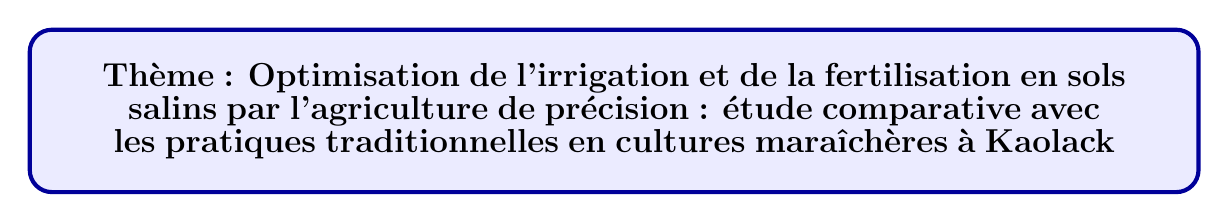
\begin{tikzpicture}
  \node[draw=blue!60!black, line width=1.5pt, rounded corners=8pt, fill=blue!8, text width=14cm, align=center, inner sep=12pt]
  {\bfseries\large Thème :  Optimisation de l’irrigation et de la fertilisation en sols salins par l’agriculture de précision : étude comparative avec les pratiques traditionnelles en cultures maraîchères à Kaolack};
\end{tikzpicture}

\vfill
\noindent
\begin{minipage}[t]{0.48\textwidth}
  \raggedright
  {\bfseries\underline{Réalisé par :}}\\[4mm]
  {\bfseries Birahim DIAGNE}\\[2mm]
  {\bfseries Mariama SANE}
\end{minipage}
\hfill
\begin{minipage}[t]{0.48\textwidth}
  \raggedleft
  {\bfseries\underline{Encadré par :}}\\[4mm]
  {\bfseries Dr. Babacar DIOP}\\[2mm]
  {\bfseries M. Mamadou L. DIEDHIOU}
\end{minipage}

\vspace{10mm}

\begin{tikzpicture}
  % aile gauche
  \filldraw[fill=white, draw=blue!50!black, line width=0.8pt]
    (-2.4,0.85) -- (-7,0.95) -- (-6.1,0.48) -- (-7,0) -- (-2.4,0.1) -- cycle;
  % aile droite
  \filldraw[fill=white, draw=blue!50!black, line width=0.8pt]
    (2.4,0.85) -- (7,0.95) -- (6.1,0.48) -- (7,0) -- (2.4,0.1) -- cycle;
  % plis gris
  \filldraw[fill=gray!40, draw=blue!50!black, line width=0.6pt]
    (-2.5,1.0) -- (-1.8,1.0) -- (-2.5,1.2) -- cycle;
  \filldraw[fill=gray!40, draw=blue!50!black, line width=0.6pt]
    (2.5,1.0) -- (1.8,1.0) -- (2.5,1.2) -- cycle;
  % cadre central
  \filldraw[fill=white, draw=blue!50!black, line width=0.8pt]
    (-2.6,-0.05) rectangle (2.6,1.0);
  \node at (0,0.475) {Année universitaire 2024--2025};
\end{tikzpicture}
\vspace{5mm}
\end{titlepage}